\documentclass[11pt]{article}
\usepackage[letterpaper,margin=0.85in]{geometry}
\usepackage{graphicx}
\usepackage{booktabs}
\usepackage{amsmath}
\usepackage{caption}
\usepackage[hidelinks]{hyperref}
\captionsetup{font=small,labelfont=bf}
\setlength{\parindent}{0pt}
\setlength{\parskip}{6pt}
\title{Lab 2: Binary Classification from Scratch\\\large Sigmoid Classifier vs. Linear SVM}
\author{COMP 395 -- Deep Learning}
\date{September 28, 2026}

\begin{document}
\maketitle
\vspace{-1.2em}

\section*{Task and methods}
This experiment classifies the 569 samples in scikit-learn's breast cancer
dataset using 30 numerical features (0 = malignant, 1 = benign). The provided
\texttt{load\_data()} function uses an 80/20 train/test split with
\texttt{random\_state=42}, giving 455 training samples and 114 test samples.
Each feature is standardized using only the training mean and standard
deviation; the same transformation is applied to the test set.

The from-scratch model is one sigmoid neuron,
$\hat y=\sigma(\mathbf{w}^{\mathsf T}\mathbf{x}+b)$, with loss
$L=\tfrac12(\hat y-y)^2$. Its gradients are computed explicitly:
\[
\delta=(\hat y-y)\hat y(1-\hat y),\qquad
\nabla_{\mathbf w}L=\delta\mathbf{x},\qquad
\frac{\partial L}{\partial b}=\delta.
\]
Weights and bias start at zero and are updated by per-sample stochastic
gradient descent with learning rate 0.01 for 100 epochs, in fixed sample
order. Predictions use a threshold of 0.5. The comparison model is
\texttt{SVC(kernel="linear", random\_state=42)}, with the default $C=1$,
trained on the same standardized training data. A linear SVM was retained
to compare a margin-based objective with squared-error training while both
models use linear decision boundaries.

\section*{Results}
The sigmoid model's average training loss decreased from 0.054478 in the
first epoch to 0.007863 in the final epoch (Figure~\ref{fig:training}).
These epoch losses average the losses observed before each sample's update.
Both models classified 449 of 455 training samples correctly.
The sigmoid classifier correctly classified 113 of 114 test samples;
the SVM correctly classified 109 (Table~\ref{tab:accuracy}).

\begin{table}[ht]
\centering
\caption{Accuracy on the same fixed train/test split.}
\label{tab:accuracy}
\begin{tabular}{lrr}
\toprule
Model & Training accuracy & Test accuracy \\
\midrule
From-scratch sigmoid classifier & 98.68\% & 99.12\% \\
Linear SVM ($C=1$) & 98.68\% & 95.61\% \\
\bottomrule
\end{tabular}
\end{table}

\clearpage
\begin{figure}[ht]
\centering
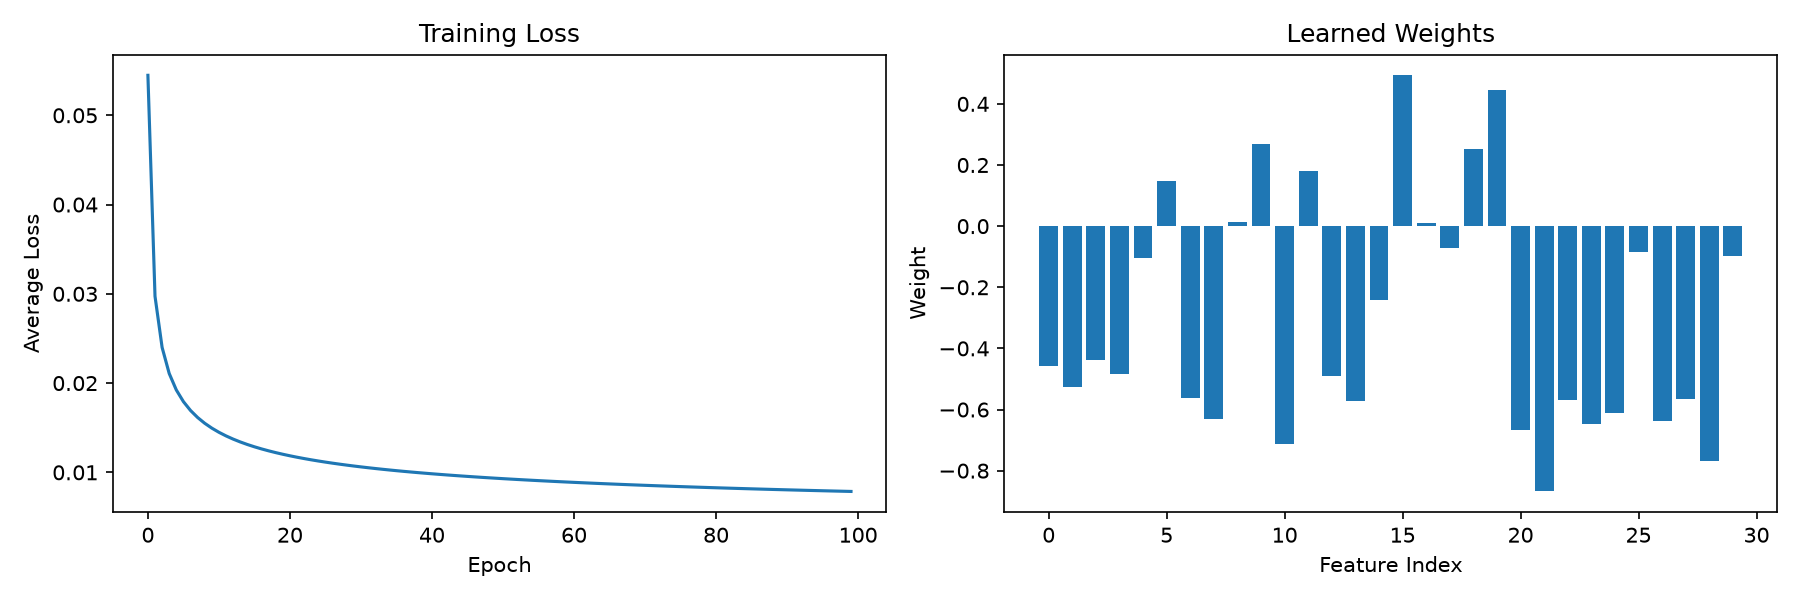
\includegraphics[width=\textwidth]{training_results.png}
\caption{Average training loss and final feature weights of the from-scratch
sigmoid classifier, generated by \texttt{binary\_classification.py}.}
\label{fig:training}
\end{figure}

\section*{Discussion}
The from-scratch classifier performed better on this test split by
3.51 percentage points, or four additional correct predictions. Both models
learn linear boundaries, but half-squared error and the SVM's margin-based
objective with regularization can select different boundaries; this is a
plausible explanation for the observed difference. It is not evidence that
the from-scratch method is generally superior: there are only 114 test
samples, no hyperparameter search was performed, and no repeated-split or
cross-validation results were collected. The measured accuracies exceed
the lab's training and test targets of 95\% and 93\%, respectively, for
the from-scratch model.

\end{document}
